\documentclass[25pt, a0paper, landscape, margin=0mm, innermargin=18mm, blockverticalspace=14mm, colspace=14mm, subcolspace=8mm]{tikzposter}
\usepackage{graphicx,booktabs,amsmath,pgfplots}\usetikzlibrary{positioning}
\pgfplotsset{compat=1.17}
\usepackage{helvet}\renewcommand{\familydefault}{\sfdefault}
\definecolorstyle{cat}{
  \definecolor{navy}{HTML}{16324F}\definecolor{sea}{HTML}{2A7FBA}\definecolor{sand}{HTML}{F4F1EA}\definecolor{coral}{HTML}{D1495B}
}{
  \colorlet{backgroundcolor}{white}\colorlet{framecolor}{navy}\colorlet{titlefgcolor}{white}\colorlet{titlebgcolor}{navy}
  \colorlet{blocktitlebgcolor}{white}\colorlet{blocktitlefgcolor}{navy}\colorlet{blockbodybgcolor}{sand}\colorlet{blockbodyfgcolor}{black}
  \colorlet{innerblocktitlebgcolor}{navy}\colorlet{innerblocktitlefgcolor}{white}\colorlet{innerblockbodybgcolor}{white}\colorlet{innerblockbodyfgcolor}{black}
  \colorlet{notefgcolor}{black}\colorlet{notebgcolor}{white}\colorlet{notefrcolor}{sea}
}
\usetheme{Simple}\usetitlestyle{Filled}
\usecolorstyle{cat}
\settitle{\centering\vbox{\color{titlefgcolor}{\fontsize{64}{76}\selectfont\bfseries \@title\par}\vspace{0.5em}{\LARGE \@author\par}\vspace{0.2em}{\large \@institute}}}
\title{Designing a 1\,m RC Foiling Beach Catamaran: CAD, Velocity Prediction, and a Build Plan}
\author{Filip Maleev}
\institute{Colorado College, Mathematics \quad | \quad September 2026}
\newcommand{\hl}[1]{{\fontsize{44}{52}\selectfont\bfseries\color{coral}#1}}
\pgfplotsset{every axis/.style={width=0.86\linewidth, height=0.58\linewidth, grid=major, grid style={gray!25}, tick label style={font=\normalsize}, label style={font=\large}, legend style={font=\normalsize, draw=none, fill=white, fill opacity=0.85, text opacity=1}}}

\begin{document}
\maketitle[width=0.97\paperwidth]
\begin{columns}

% ------------------------------------------------------------------ column 1
\column{0.25}
\block{The question}{
Can a 3D-printed 1\,m radio-controlled catamaran look and sail like a real beach cat (Hobie~16, Nacra~17), \textbf{fly on hydrofoils}, and still be \textbf{controllable}? The answers had to be known before building.
\vspace{0.6em}
\begin{center}
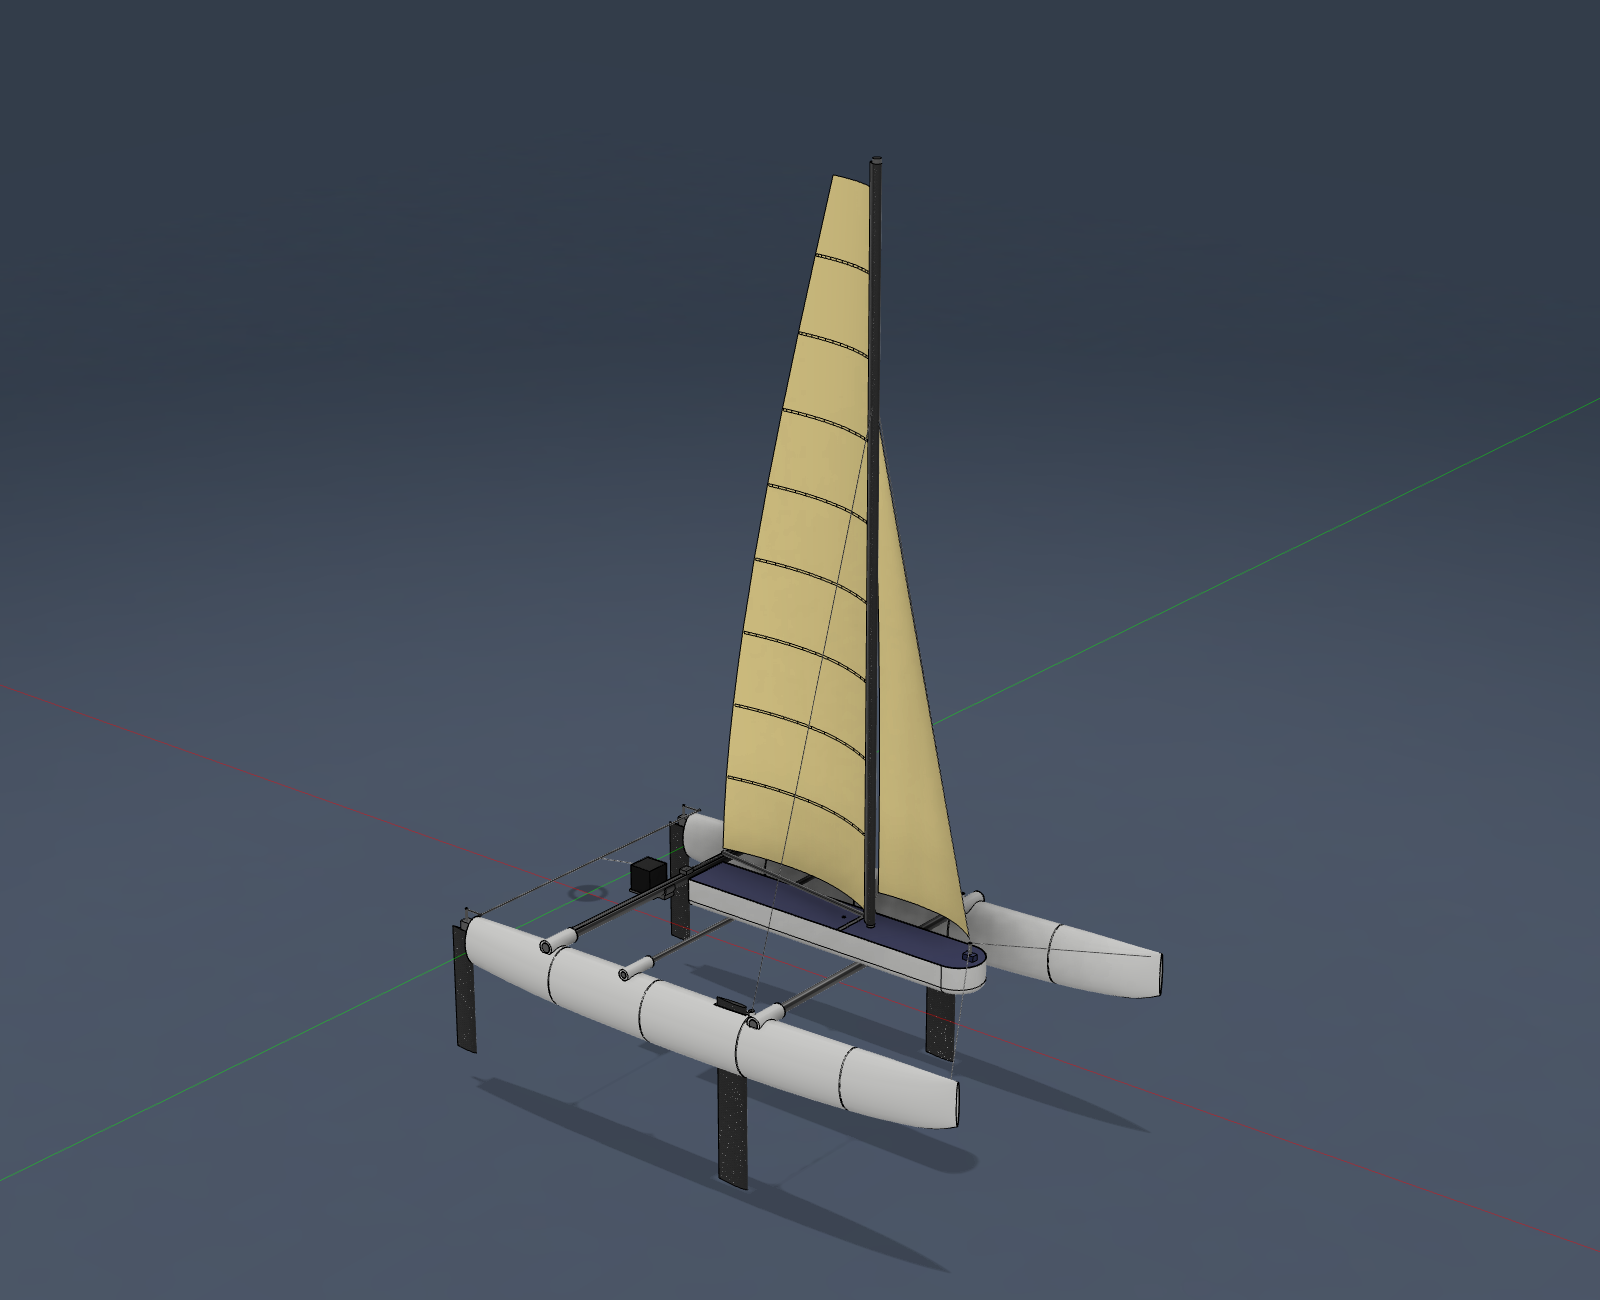
\includegraphics[width=0.46\linewidth]{../images/build_first_v1.4.png}\hfill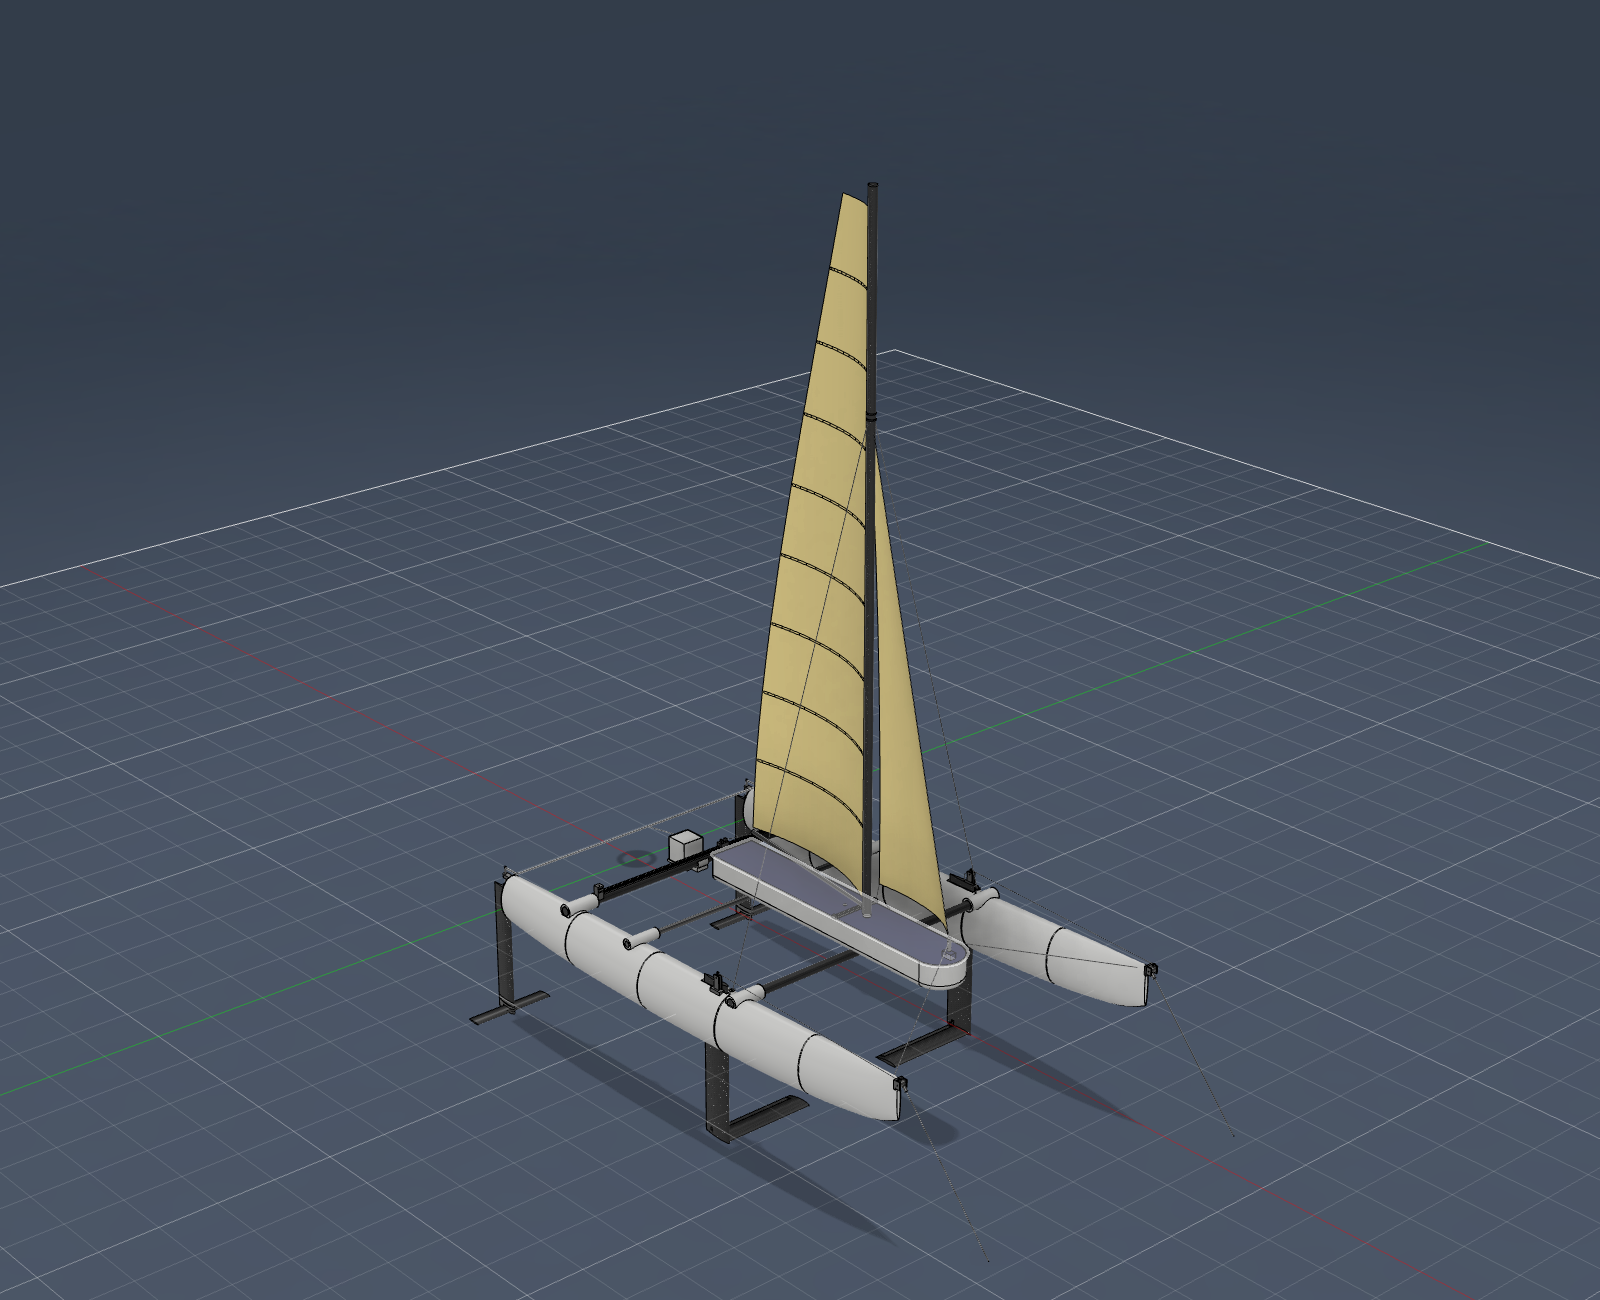
\includegraphics[width=0.46\linewidth]{../images/foiling_v2.3.png}\\
{\normalsize Build-first version (daggerboards) \hfill Foiling version (v2.3 L-foils, T-foil rudders)}
\end{center}
}
\block{Design (Autodesk Fusion, scripted through its API)}{
\begin{itemize}
\item \textbf{Hulls:} 8 elliptical stations, 1000\,mm, printed as 0.8\,mm PETG shells. Bulkheads bonded in at every print joint make each segment \textbf{a sealed compartment}.
\item \textbf{Rig from real cats:} square-top main with 8 full-length battens, rotating wing mast, forestay bridle, traveler and jib car.
\item \textbf{Scale effect:} righting moment $\propto \lambda^4$ but heeling moment $\propto \lambda^3$, so sail area was sized by analysis, not by geometric scaling.
\end{itemize}
\vspace{0.3em}
\begin{center}
\begin{tabular}{lccc}
\toprule
 & Hobie 16 & Nacra 17 & \textbf{This boat} \\
\midrule
Mast / LOA & 1.60 & 1.71 & \textbf{1.37} \\
Main : jib & 2.7 & 3.7 & \textbf{3.2} \\
Sail area / LOA$^2$ & 0.74 & 0.68 & \textbf{0.40} \\
\bottomrule
\end{tabular}
\end{center}
}
\block{Sail trim on sliders}{
\begin{minipage}[c]{0.6\linewidth}
A custom Fusion add-in maps the three real-cat controls to three sliders and three RC servos: \textbf{jib sheet}, \textbf{main traveler}, and \textbf{mainsheet tension} (twist 30$^\circ\!\to\!3^\circ$, depth 13\,\%\,$\to$\,8\,\%). The sails are parametric lofts that re-solve as you slide.\\[0.4em]
{\normalsize Right: reaching trim seen from above, boom eased 25$^\circ$, the top of the main twisted off.}
\end{minipage}\hfill
\begin{minipage}[c]{0.36\linewidth}\centering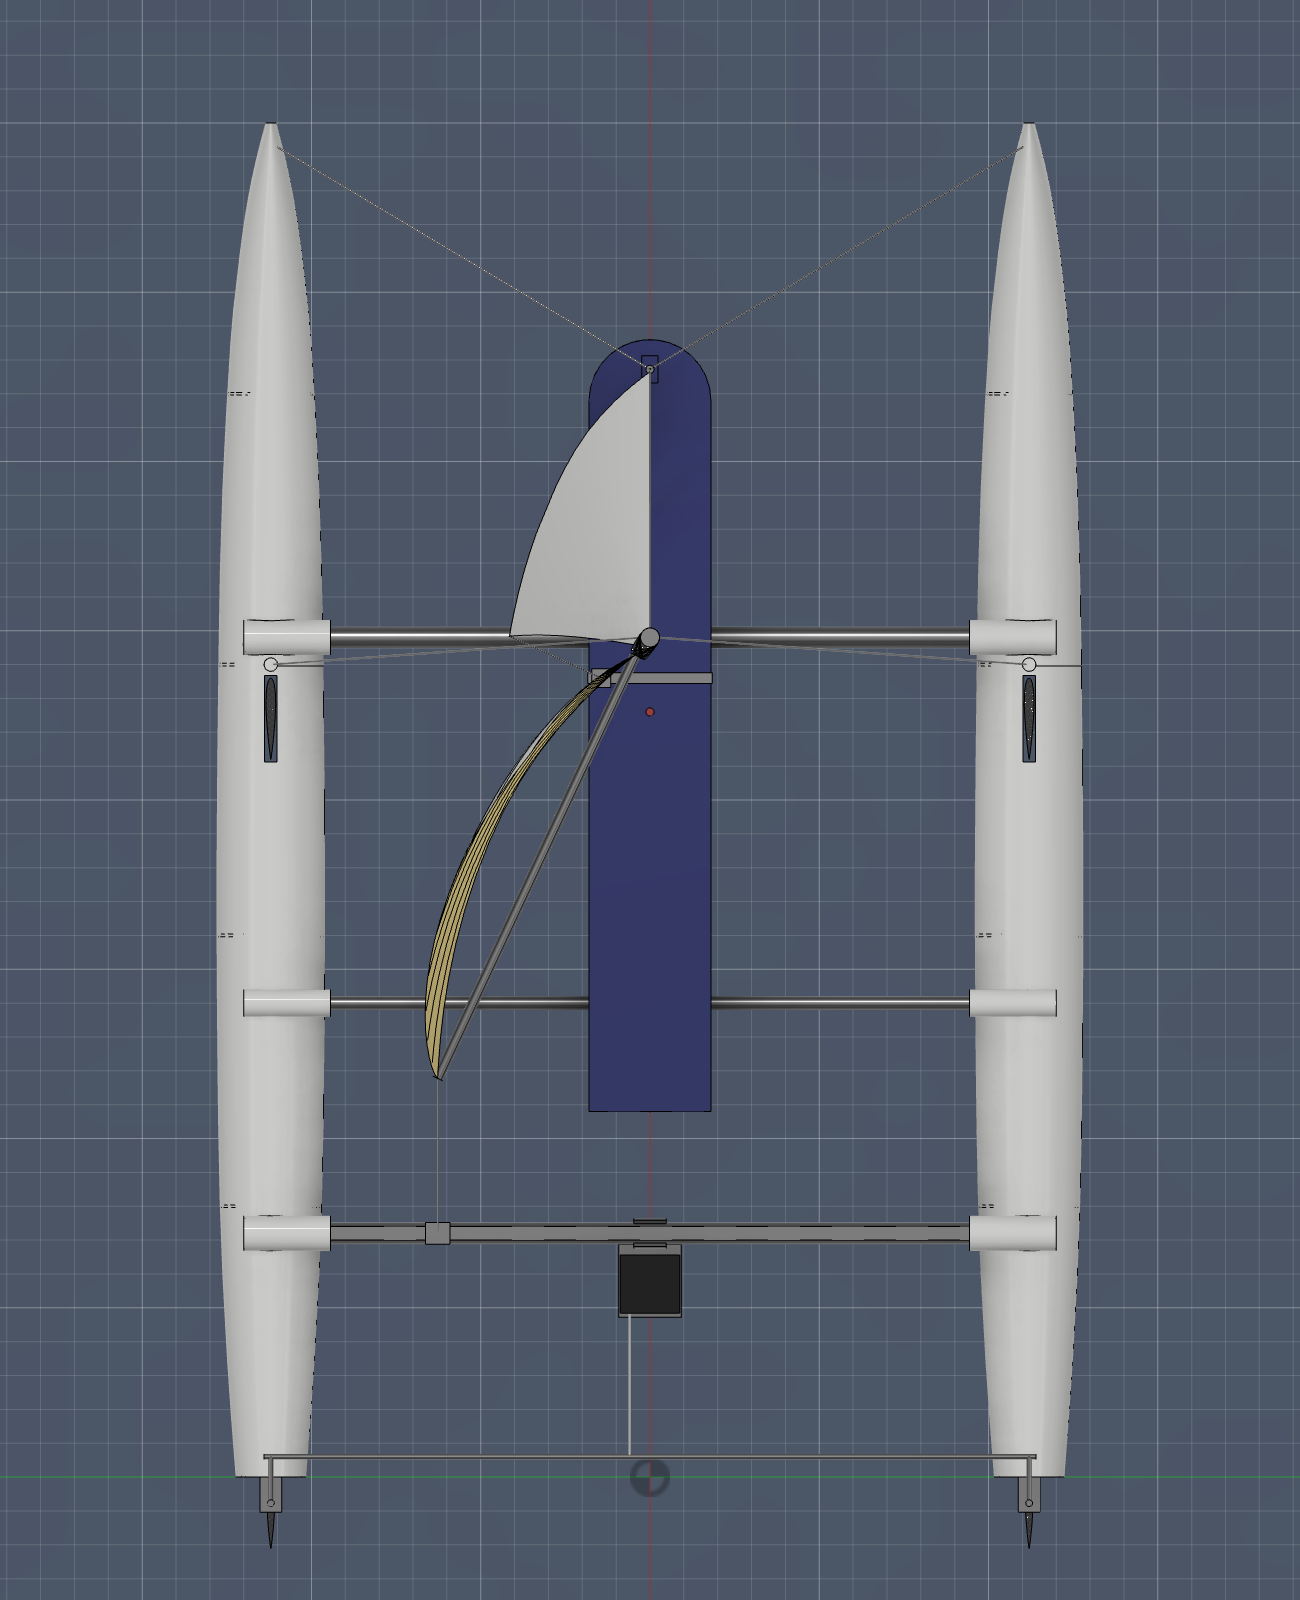
\includegraphics[height=11cm]{../images/trim_reaching_top.png}\end{minipage}
}

% ------------------------------------------------------------------ column 2
\column{0.25}
\block{Method: a purpose-built velocity prediction program}{
\begin{center}
\begin{tikzpicture}[node distance=9mm, box/.style={draw=navy, fill=white, rounded corners, text width=0.72\linewidth, align=center, inner sep=5mm, font=\large}]
\node[box] (a) {CAD geometry + mass properties (Fusion API)};
\node[box, below=of a] (b) {Hydrostatics: station integration (0.20\,\% of CAD volume)};
\node[box, below=of b] (c) {Resistance: ITTC-57 friction + \textbf{Michell wave integral} + appendages};
\node[box, below=of c] (d) {Foil lift: thin-airfoil $\alpha_{L0}$ + lifting line};
\node[box, below=of d] (e) {Sails: $C_L, C_D$ model, flattened to stay under 90\,\% of righting moment};
\node[box, below=of e, fill=sea!15] (f) {\textbf{VPP}: speed where drive = drag; controllability checks};
\foreach \u/\v in {a/b,b/c,c/d,d/e,e/f} \draw[-latex, very thick, navy] (\u) -- (\v);
\end{tikzpicture}
\end{center}
\vspace{0.4em}
Michell's thin-ship integral, with a catamaran interference factor $F_c$:
\[ R_W=\frac{4\rho g^2}{\pi U^2}\int_1^\infty \big(I^2+J^2\big)\frac{\lambda^2F_c(\lambda)}{\sqrt{\lambda^2-1}}\,d\lambda \]
\[ F_c=4\cos^2\!\Big(\tfrac{g}{U^2}\lambda\sqrt{\lambda^2-1}\,\tfrac{s}{2}\Big) \]
Integrated exactly in $x$ and $z$ on each panel (Filon-type), so it stays accurate at low Froude numbers.
}
\block{Validation}{
\begin{center}
\begin{tikzpicture}
\begin{axis}[xlabel={Froude number}, ylabel={$10^3\,C_W$ (Wigley hull)}, ymin=0, height=0.45\linewidth, xtick={0.2,0.3,0.4,0.5,0.6}]
\addplot[ultra thick, sea] table[x=Fn, y=Cw] {../paper/data/wigley.dat};
\end{axis}
\end{tikzpicture}
\end{center}
Grid refinement changes the result by less than \textbf{0.03\,\%}, and the hump at $Fn\approx0.3$ and the main hump at $Fn\approx0.5$ both appear. A hull-drag regression test guards every code change.
}

% ------------------------------------------------------------------ column 3
\column{0.25}
\block{Results: speed and take-off}{
\begin{center}
\begin{tikzpicture}
\begin{axis}[xlabel={True wind (kn)}, ylabel={Boat speed (m/s)}, legend pos=south east, xmin=3, xmax=16, ymin=0]
\addplot[ultra thick, sea, mark=*] table[x=tws, y=V] {../paper/data/vpp_displacement_90.dat}; \addlegendentry{build-first, beam reach}
\addplot[ultra thick, coral, mark=square*] table[x=tws, y=V] {../paper/data/vpp_foiling_90.dat}; \addlegendentry{foiling, beam reach}
\end{axis}
\end{tikzpicture}
\end{center}
\begin{itemize}
\item Build-first: \hl{2.6\,m/s} in 8\,kn of wind on a beam reach.
\item Foiling: takes off at \textbf{1.8\,m/s} from about \textbf{7.1\,kn}, below the 8--9\,kn where the rig must be depowered.
\item Sensitivity (sail $C_L$ $\pm$15\,\%, foil lift $-$20\,\%, mass $\pm$10\,\%, sail-drive couple $\times$0.5--1.5, laminar foil friction): take-off between \textbf{6.25 and 11\,kn}.
\end{itemize}
}
\block{Results: can it be controlled?}{
\begin{itemize}
\item \textbf{Rudders (build-first):} need at most \hl{2.6$^\circ$} of $\pm$18$^\circ$ throw, with $\geq$77\,\% margin to stall, even with the windward rudder out of the water.
\item \textbf{Foil pitch:} stable, with the CG 41--97\,mm ahead of the neutral point.
\item \textbf{Bows (pitchpole):} v1.3 hulls add forward volume: +23\,\% bow-down margin for +0.4\,\% drag. The VPP now eases the sails for pitch as well as heel.
\item \textbf{Foil heave: NOT stable.} Fixed-angle foils lift \hl{+120\,\%} more than the boat's weight at 4\,m/s, so the boat would climb, breach and crash.
\end{itemize}
\begin{center}
\begin{tikzpicture}
\begin{axis}[xlabel={Boat speed (m/s)}, ylabel={Lift beyond weight (\%)}, height=0.3\linewidth, xtick={2,2.5,3,3.5,4}]
\addplot[ultra thick, coral, mark=*] table[x=V, y=excess] {../paper/data/heave.dat};
\end{axis}
\end{tikzpicture}
\end{center}
\textbf{v2 fix, sized:} a bow wand on each hull drives a 25\,\%-chord flap on that hull's foil. Heave becomes stable and over-damped ($\zeta$\,=\,1.6, 2.2--5.8\,Hz) using at most 10.2$^\circ$ of flap across the flying range. \textbf{Build order:} mini, then the 1\,m boat without foils, then foils with wands.
}

% ------------------------------------------------------------------ column 4
\column{0.25}
\block{First build: RC Mini Cat 600}{
\begin{center}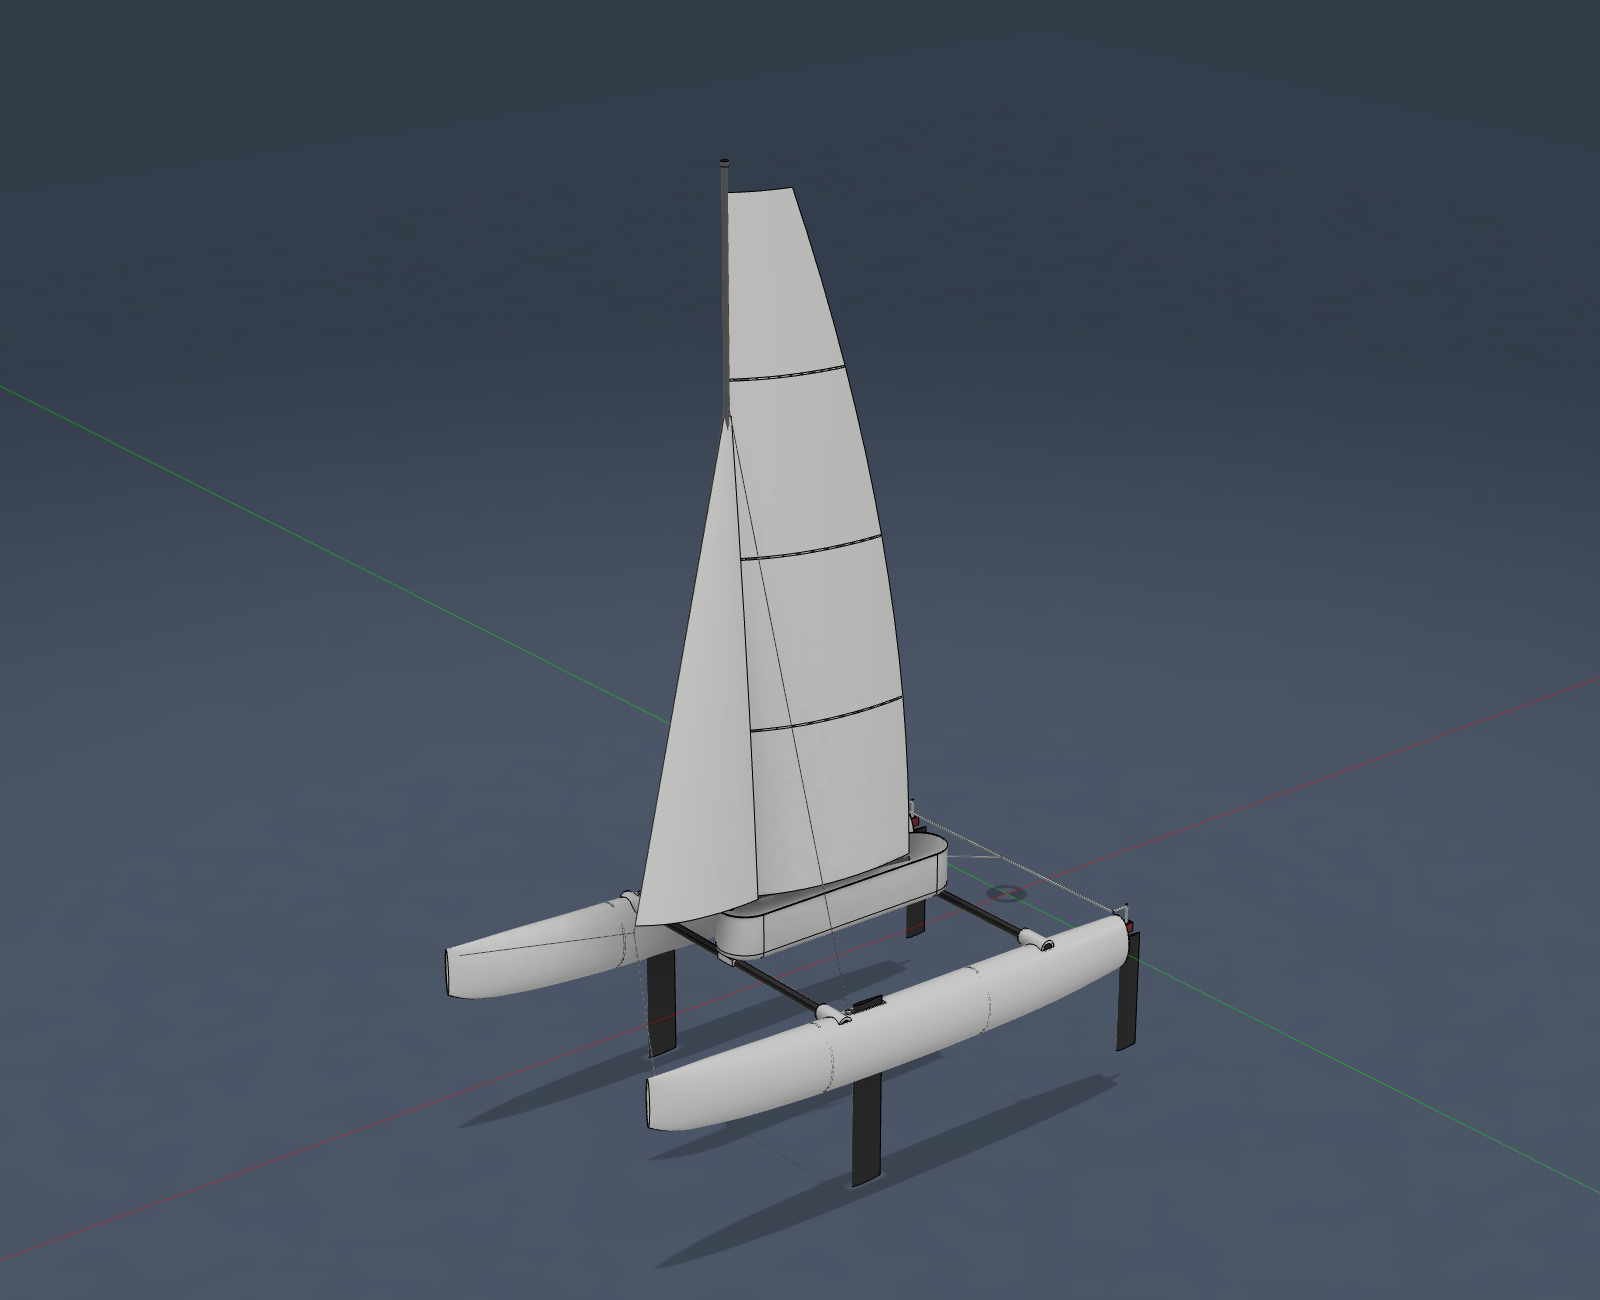
\includegraphics[width=0.4\linewidth]{../mini/images/mini_iso.png}\end{center}
Same lines, rig and printed construction at 0.6 length, but hull sections scaled 0.68, because the electronics do not shrink. One winch with a \textbf{stepped drum} (30 / 16.2\,mm) pulls both sheets, sized so both reach full ease in the same 1.63 turns.
\begin{itemize}
\item 755\,g sailing weight; one hull alone floats 2.05$\times$ its weight
\item 2.1\,m/s predicted in 8\,kn; at most 1.6$^\circ$ of rudder needed
\end{itemize}
}
\block{What it costs (USD, prices read 23-24 Sep 2026)}{
\begin{center}
\begin{tikzpicture}
\begin{axis}[xbar, xmin=0, height=0.4\linewidth, xtick={0,20,40,60,80}, symbolic y coords={{Servos},{Printed},{Rigging},{Power},{Adhesives},{Hardware},{Sails},{Carbon},{Radio}}, ytick=data, xlabel={USD}, nodes near coords, nodes near coords align={horizontal}, nodes near coords style={font=\normalsize, /pgf/number format/fixed, /pgf/number format/precision=0}, bar width=16pt, enlarge y limits=0.08, xmax=95]
\addplot[fill=sea, draw=navy] coordinates {(13.72,{Servos}) (13.99,{Printed}) (14.43,{Rigging}) (16.75,{Power}) (18.78,{Adhesives}) (20.52,{Hardware}) (42.84,{Sails}) (43.36,{Carbon}) (72.98,{Radio})};
\end{axis}
\end{tikzpicture}
\end{center}
\centering\hl{\$257.37} in parts for the mini\quad|\quad \textbf{\$381.02} for the 1\,m boat (+\$101.17 foils)\par
{\normalsize Every price was read on a retailer page. The build manual has the full list, 1:1 sail patterns and 10 build steps.}
}
\block{Checked in CAD, next on the water}{
\begin{itemize}
\item Servo rails redrawn from the makers' drawings.
\item A 9-trim clearance sweep moved the pod forward onto a light third beam. Every fitting is now drawn and printable.
\item Flight simulator with pitch trim, 306{,}180 foil designs: positive-incidence elevators would pitch the boat nose-down and out of the water. \textbf{v2.3} (in CAD): elevators at $-0.5^\circ$, 18\,mm lower; flies level at 12\,kn.
\item \textbf{Next:} build the mini, then the 1\,m boat; tow-test the v2.3 foils, then fly.
\end{itemize}
}
\end{columns}
\end{document}
